\documentclass[oneside,10pt,a4paper]{scrartcl}
\usepackage{pdfpages}
\usepackage{ngerman}
\usepackage{algorithmic}
\usepackage{fancyhdr}
\usepackage{listings}
\RequirePackage[utf8]{inputenc}
\usepackage[T1]{fontenc}
\usepackage{graphicx}
\usepackage{url}
\usepackage{listings}

\lstset{numbers=left,numberblanklines=false,basicstyle=\ttfamily,xleftmargin=0pt}
\addtolength{\oddsidemargin}{-0.25\marginparwidth}

\renewcommand{\sectionmark}[1]{\markboth{\thesection\ #1}{}}
\lhead[ \leftmark   ]{\textbf{Einkaufsoptimierung}}
\rhead[]{Kai Fabian, Dominik Moritz, Matthias Springer, Malte Swart}
\cfoot[\thepage]{\thepage}

\begin{document}
\begin{titlepage}
\author{Kai Fabian\\Hasso-Plattner-Institut, IT-Systems Engineering, 3. Semester\\\texttt{kai.fabian@student.hpi.uni-potsdam.de} 
\and Dominik Moritz\\Hasso-Plattner-Institut, IT-Systems Engineering, 3. Semester\\\texttt{dominik.moritz@student.hpi.uni-potsdam.de}
\and Matthias Springer\\Hasso-Plattner-Institut, IT-Systems Engineering, 3. Semester\\\texttt{matthias.springer@student.hpi.uni-potsdam.de}
\and Malte Swart\\Hasso-Plattner-Institut, IT-Systems Engineering, 3. Semester \\\texttt{malte.swart@student.hpi.uni-potsdam.de}}

\title{
\includegraphics{resourcen/logo.png}\\ShoppingTour}
\subtitle{Einkaufsoptimierung\\informatiCup 2012 Aufgabe 1}

\date{\today}
\maketitle
\end{titlepage}
\pagestyle{fancy}
\tableofcontents

\section{Installation}
Windows-Nutzer können weitgehende Installationsschritte durch die Verwendung unserer \emph{Windows One-Click Distribution} in der beigelegten Datei \texttt{shoppingtour-w32.zip} vermeiden. Hierzu wird diese Datei in einen beliebigen Ordner entpackt und die enthaltene \texttt{shoppingtour.exe}-Datei ausgeführt.

Da dieses Projekt ausschließlich in der plattformunabhängigen Skriptsprache \emph{Python} geschrieben wurde, ist eine Distribution auf fast alle Betriebssysteme möglich. Notwendige Voraussetzung hierfür ist jedoch, dass die im Projekt verwendeten notwendigen Bibliotheken für das Zielsystem verfügbar sind. Da dies meist nur für verbreitete Betriebssysteme der Fall ist, können wir eine Lauffähigkeit zum aktuellen Zeitpunkt nur für \emph{Microsoft Windows} (2000, XP, Vista, 7, 8 Developer Preview), \emph{Apple Mac OS X} (>= 10.4) und \emph{Linux} (Kernel 2.6/3.0, insbesondere Distributionen ''Debian'', ''Ubuntu'' und ''Gentoo'') garantieren.

Im Folgenden werden die notwendigen Softwarepakete aufgeführt, die für die Verwendung von \emph{ShoppingTour} erforderlich sind.

\subsection{ShoppingTour}
\url{http://www.myhpi.de/~kai.fabian/shoppingtour/}

ShoppingTour benötigt keine Installation und kann nach dem Entpacken in ein beliebiges Verzeichnis, welches das Ausführen von Anwendungen erlaubt, verwendet werden.

\subsection{Python 2.7}
\url{http://www.python.org/}

Als Interpreter für die verwendete Programmiersprache empfehlen wir die Referenzimplementierung \emph{CPython} in der \emph{Version 2.7}, wobei auch andere kompatible Python-Implementierungen verwendbar sein sollten, solange die weiteren Abhängigkeiten Kompatibilität zu diesen aufweisen.

Bezüglich der Python-Prozessorarchitekturen konnten die Intel 32-bit-Architektur (x86) sowie die AMD 64-bit-Architektur (x64) erfolgreich erprobt werden.

\subsection{PyQt 4.9}
\url{http://www.riverbankcomputing.co.uk/software/pyqt/download}

Das Benutzer-Interface verwendet Nokias Qt-Bibliothek. Die hierfür notwendigen Python-Bindungen werden durch Riverbank Computing Limited bereitgestellt. Für Windows existieren vorkompilierte Pakete, während Linux- und Mac-Nutzer die Bibliothek selbst kompilieren müssen, sofern nicht bereits vorgefertigte Pakete für das Betriebssystem existieren (bspw. das Paket \texttt{py27-pyqt4} für Mac OS X unter Verwendung von MacPorts).

Anzumerken ist hierbei, dass zur Verwendung (und eventuellen manuellen Übersetzung) der PyQt-Bibliothek Nokias Qt-Bibliothek neben weiteren Abhängigkeiten (hierzu sei an die Seiten des PyQt-Distributors verwiesen) auf dem System vorhanden sein müssen.

\subsection{Clingo (part of Potassco)}
\url{http://potassco.sourceforge.net/}

Das von der Universität Potsdam gepflegte Potassco-Projekt stellt Softwarewerkzeuge für ASP-Programmierung (Answer Set Programmung) bereit. \emph{ShoppingTour} verwendet \emph{Clingo}, welches die Verbindung von clasp, einem Lösungsproblem für logische Probleme, und Gringo, einem Konvertierer zur Erzeugung von variablen-freien logischen Problembeschreibungen, darstellt. Vorkompilierte Binärdateien für Windows, Mac OS/Darwin und Linux sind von der Anbieterseite ebenso zu erhalten wie der Software-Quellcode.

\newpage

\section{Programmverwendung}


\subsection{Verwendung der graphischen Ansicht}

Nach dem Programmstart befindet sich der Benutzer üblicherweise in der graphischen Ansicht.

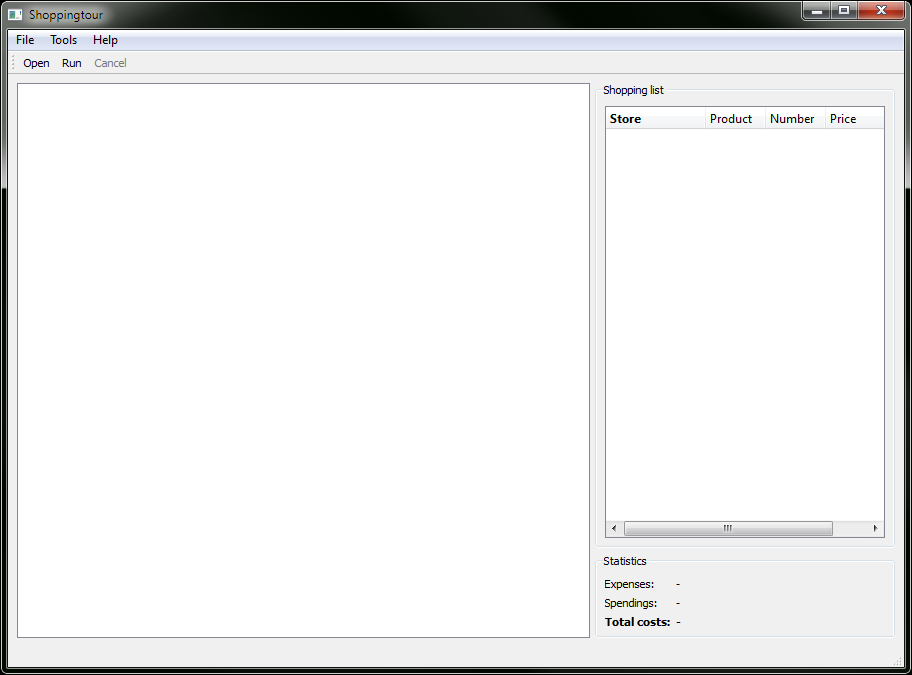
\includegraphics[width=1\textwidth]{resourcen/walkthrough/0-default-view.png}

\newpage

Der Benutzer öffnet nun eine Problemdefinition, in dem er den \emph{Open}-Button in der Toolbar, oder wahlweise den gleichnamigen Menüpunkt im File-Menü, verwendet. Hierbei hat er die Wahl zwischen den beiden implementierten Algorithmen.

In der folgenden Ansicht wählt der Benutzer die Problembeschreibungsdateien über den \emph{Select}-Button oder durch manuelle Eingabe in das Textfeld aus.

Für die Verwendung von Clingo zur Problemlösung muss der Pfad zur ausführbaren Programmdatei angegeben werden. In der \emph{Windows One-Click Distribution} befinden sich diese im dist/clingo-Ordner; Windows-Benutzer müssen hier also den Pfad zur \texttt{w32clingo.exe}-Datei, also beispielsweise \texttt{dist/clingo/w32clingo.exe}, angeben. Der Pfad kann hierbei absolut oder relativ zum aktuellen Arbeitsverzeichnis angegeben werden.

Alternativ kann der Benutzer den genetischen Algorithmus wählen. Hierbei kann er die Eckdaten des Algorithmenverhaltens bestimmen. Die Beschreibung der Buttonfunktionen kann über den \emph{Help}-Button erfahren werden.

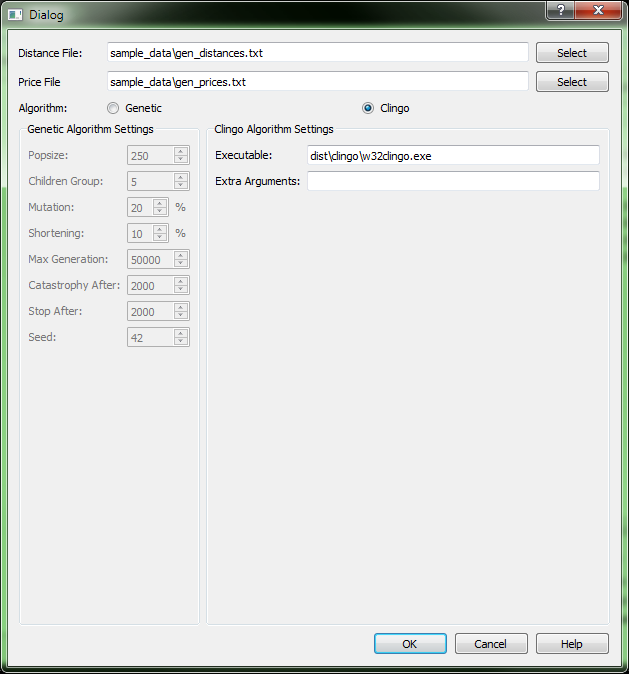
\includegraphics[width=0.48\textwidth]{resourcen/walkthrough/1a-open-clingo.png} 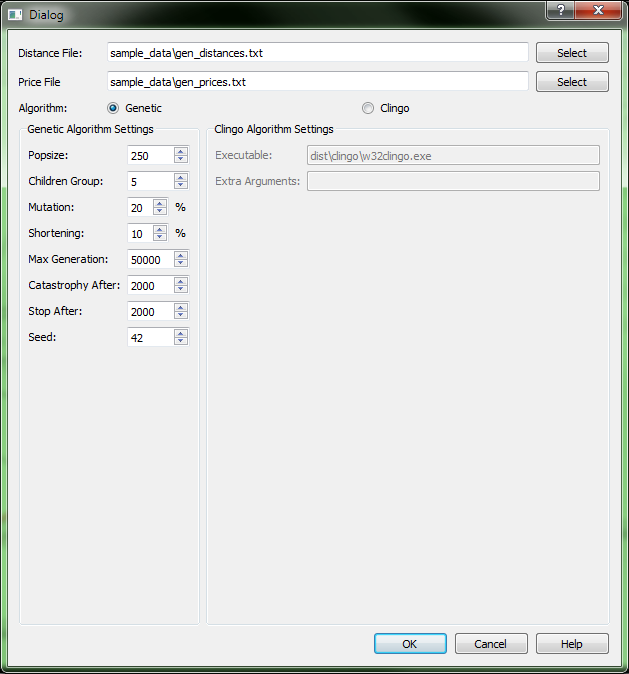
\includegraphics[width=0.48\textwidth]{resourcen/walkthrough/1b-open-genetic.png}

\newpage

Der Benutzer sieht nun eine graphische Darstellung des Problembereiches. Er kann per Klicken und Ziehen die einzelnen Knoten des Graphen verschieben (optional kann er die Funktion der elastischen Knoten im ''Tools''-Menü aktivieren).

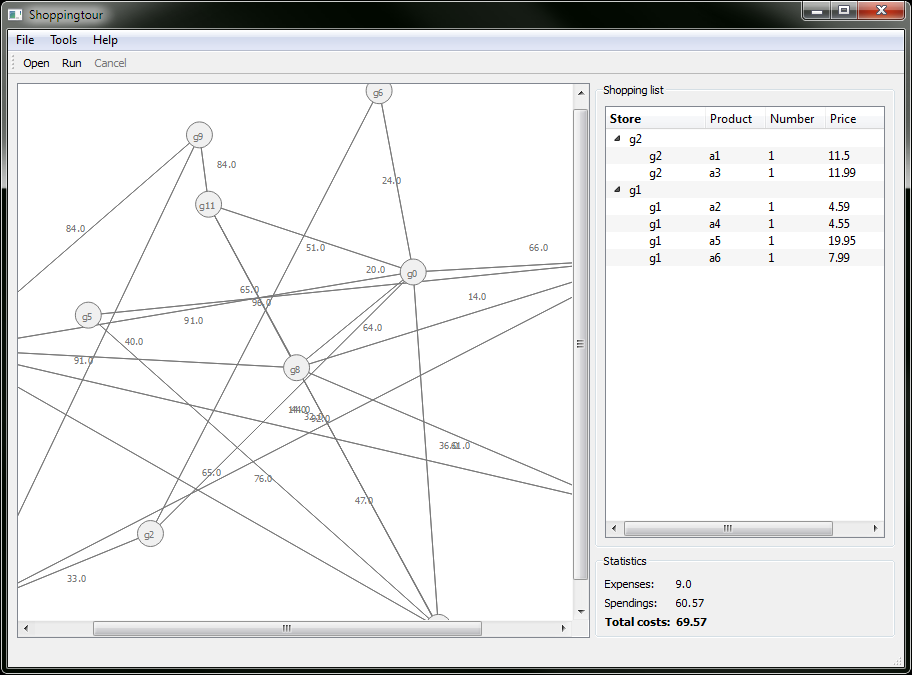
\includegraphics[width=1\textwidth]{resourcen/walkthrough/2-opened-clingo.png}

\newpage

Um die Berechnung zu starten, klickt der Benutzer auf den \emph{Run}-Button in der Toolbar. Während des Algorithmen-Durchlaufs wird ihm der aktuelle Programmzustand, also die aktuell berechnete (Teil-) Lösung, graphisch und in Listenform dargestellt.

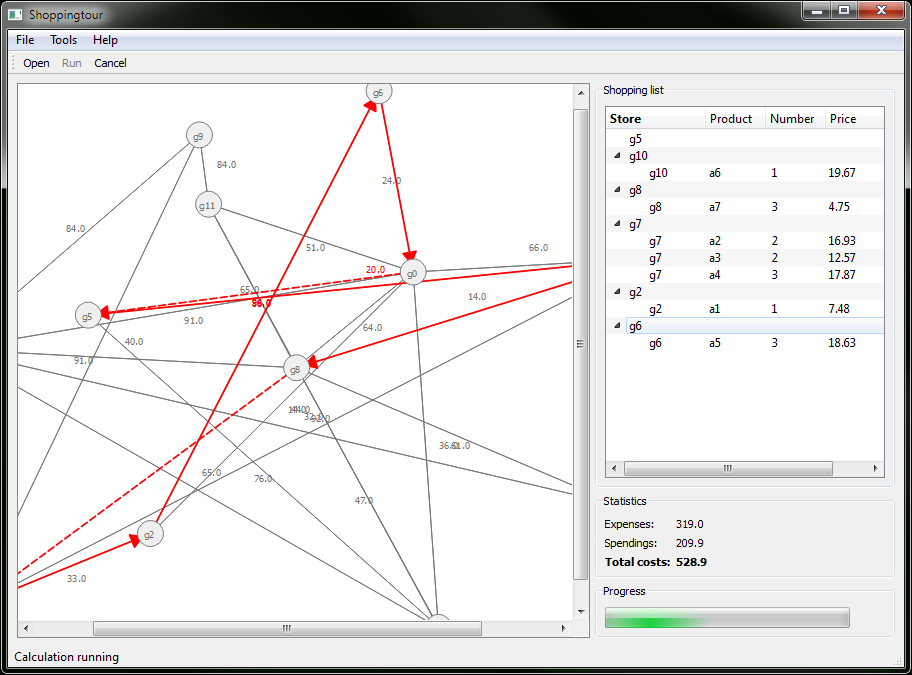
\includegraphics[width=1\textwidth]{resourcen/walkthrough/3-running-clingo.png}

\newpage

Der Benutzer kann den Berechnungsvorgang selbstverständlich auch abbrechen. Hierzu wählt er entweder in der Toolbar die \emph{Cancel}-Option oder alternativ die gleichnamige im Tools-Menü.

In der Endansicht wird der Benutzer über die beste gefundene Lösung informiert. Dies geschieht auch hier einerseits in graphischer Form und andererseits in Listenform. Die Listenform wird als \emph{Shopping list} bezeichnet und beschreibt, in welcher Reihenfolge welche Geschäfte besucht werden sollen (erste Baumebene) und welche Gegenstände in welcher Anzahl dort gekauft werden sollen (zweite Baumebene).

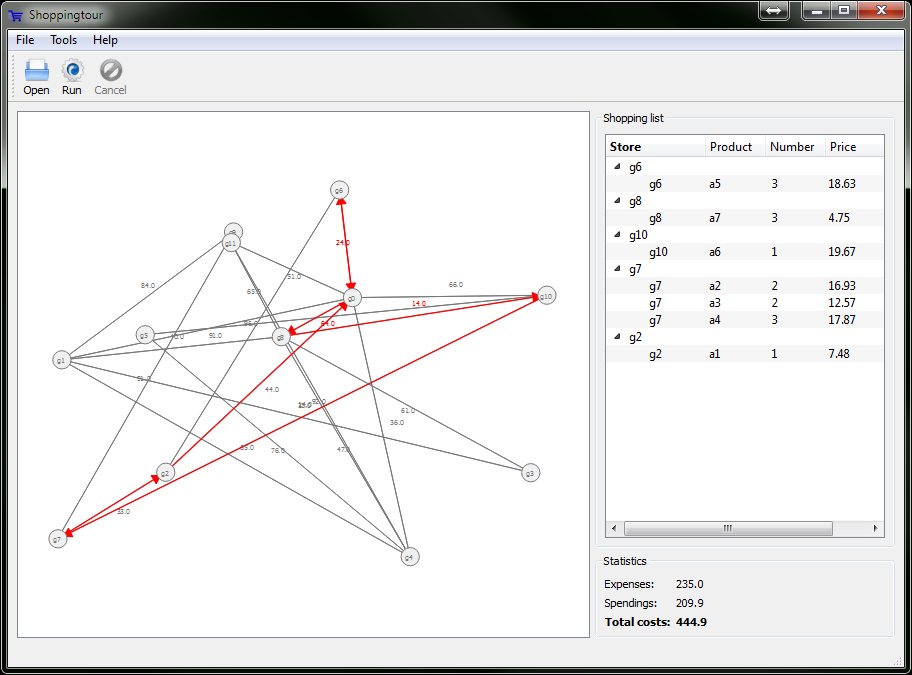
\includegraphics[width=1\textwidth]{resourcen/walkthrough/4-finished-clingo.png}

\newpage
\section{Ein NP-schweres Problem}
Bei dem vorliegenden Problem handelt es sich um NP-schweres Problem. Das ist deshalb interessant, weil es somit nahezu ausgeschlossen ist, einen Algorithmus zu finden, der die optimale Lösung des Problems effizient (in polynomieller Zeit) berechnet. Durch polynomielle Reduktion des \emph{Travelling Salesman Problems} (TSP) auf das vorliegende Problem kann die NP-Schwierigkeit gezeigt werden.

Beim TSP geht man von einem ungerichteten, gewichteten Graphen aus, wobei die Knoten des Graphen Städte und die Kanten des Graphen Verkehrswege zwischen den Städten repräsentieren. Das Gewicht einer Kante gibt Aufschluss ¸ber die Länge des Weges zwischen zwei Städten. Nun soll eine Rundreise, also ein Pfad mit dem gleichen Start- und Endknoten, mit dem kleinstmˆglichen Reiseweg gesucht werden, wobei alle St‰dte einmal besucht werden m¸ssen.

Das TSP lässt sich auf das Problem der Einkaufsplanung reduzieren, indem man den Graphen ohne Veränderung übernimmt\footnote{Einkaufsgeschäfte sind Städte.}. Wenn $S=\{s_1, s_2, \ldots\}$ die Menge der Städte ist, erzeugen wir für jede Stadt $s_i$ einen Artikel $a_i$, den es nur in dieser Stadt zu kaufen gibt. F¸r die letzte Stadt $s_n$ gibt es keinen Artikel, denn das soll unser Start- und Endpunkt sein, an dem die Reise beginnt. Der Preis der Artikel spielt keine Rolle, solange er endlich ist, also setzen wir ihn einfach auf $0$.

Jeder Artikel soll nun einmal eingekauft werden. Durch die Lösung des Einkaufsplanungsproblems erhalten wir eine optimale Lösung des TSP, denn es werden die Gesamtkosten minimiert, die in diesem Fall nur aus den Reisekosten bestehen. Die Reisekosten aber ist die Länge der Rundreise. Um jeden Artikel einzukaufen, muss des weiteren jede Stadt einmal besucht werden. Als Ergebnis erhalten wir u.a. die Reihenfolge, in der die Städte besucht werden sollen, was der Lösung des TSP entspricht. Die Transformation des Problems ist trivialerweise in polynomieller Zeit möglich, denn es muss lediglich für jede Stadt ein Artikel erstellt werden (linearer Zeitaufwand).

Um zu zeigen, dass es sich außerdem um ein NP-vollständiges Problem handelt, muss nachgewiesen werden, dass das Problem in der Menge NP enthalten ist. Es muss also gezeigt werden, dass eine Lösung in polynomieller Zeit verifiziert werden kann. An dieser Stelle soll nur das Entscheidungsproblem betrachtet werden: Gibt es eine Lösung des des Einkaufsplanungsproblems, deren Gesamtkosten unter dem Betrag $n$ liegen? Eine mögliche Lösung kann durch Aufsummieren der Reisekosten zwischen den Einkaufsläden\footnote{Die Reisekosten ergeben sich aus den Kantengewichten.} und dem Addieren der Artikelpreise bei den entsprechenden Einkaufsläden in polynomieller Zeit\footnote{Wie man sich leicht überlegen kann, macht es keinen Sinn, eine Kante mehr als zweimal zu benutzen.} verifiziert werden. Somit handelt es sich um ein NP-schweres Problem, das selbst in NP liegt, also folglich um ein NP-vollst‰ndiges Problem.

\section{Pre- und Postprocessing}
Um die Implementierung unserer Algorithmen zu verbessern und den Zustandsraum zu verkleinern, wird vor der Ausf�hrung ein Preprocessing-Schritt und nach der Ausf�hrung ein Postprocessing-Schritt durchgef�hrt.

\subsection{Preprocessing}
Als Eingabe erh�lt das Programm u.a. eine Adjazenzmatrix eines gewichteten, ungerichteten Graphen, in dem die Gesch�fte auf Knoten und die Wege zwischen den Gesch�ften auf Kanten abgebildet werden. Das Gewicht einer Kante ist der Abstand zwischen zwei Gesch�ften bzw. die Kosten, die bei der Fahrt entstehen. Es ist auch m�glich, dass zwischen Gesch�ften gar keine Verbindung existiert, was entweder bedeutet, dass das Gesch�ft nur �ber ein anderes Gesch�ft erreichbar ist, oder dass der Graph nicht zusammenh�ngend ist. 

Falls der Graph nicht zusammenh�ngend ist, k�nnen die Knoten, die nicht vom Start- und Endknoten aus erreichbar sind, einfach verworfen werden. Diese sind dann n�mlich nicht relevant f�r die Berechnung, weil sie in keiner validen L�sung auftauchen k�nnen. Sie w�rden den Suchraum nur unn�tig vergr��ern. Nicht erreichbare Knoten k�nnen mit einer Tiefensuche in linearer Zeit\footnote{$\mathcal{O}(|V|+|E|)$, wobei $|V|$ die Anzahl der Knoten und $|E|$ die Anzahl der Kanten ist.} gefunden und gel�scht werden.

Die eigentlichen Algorithmen entscheiden nur, ob und in welcher Reihenfolge bestimmte Knoten angesteuert werden sollen. Es wird also nicht direkt betrachtet, welchen Preis die Einkaufsartikel haben. Die L�sung, die ein Algorithmus generiert, ist nur eine Liste mit den anzusteuernden Knoten. Welche Artikel bei welchem Gesch�ft gekauft werden, muss nicht gespeichert werden. Dazu geht man einfach alle Artikel durch ein w�hlt f�r jeden Artikel das Gesch�ft unter den besuchten Gesch�ften aus, das den Artikel zum niedrigsten Preis anbietet. 

Eine solche Rundreise kann aber sehr gro� sein, da es passieren kann, dass ein Gesch�ft mehrmals besucht werden muss\footnote{Man denke z.B. an einen Fall, wo ein Gesch�ft A nur �ber ein einziges anderes Gesch�ft B erreichbar ist. Dann muss man dieses Gesch�ft B mindestens zweimal besuchen, einmal um zu A zu gelangen und einmal um A wieder zu verlassen. Analog lassen sich F�lle konstruieren, bei denen ein Gesch�ft beliebig oft besucht werden muss.}. Durch eine Optimierung im Preprocessing kann der Suchraum aber stark verkleinert werden.

Dazu wird der Graph in einen vollst�ndigen Graphen umgewandelt. Jeder Knoten ist dann von jedem anderen Knoten aus direkt erreichbar. Als Kantengewicht einer hinzugef�gten Kante w�hlt man den minimalen Abstand zwischen den beiden betroffenen Knoten. In einem solchen Graphen muss kein Knoten mehr als einmal besucht werden. Um einen Artikel in einem bestimmten Gesch�ft zu kaufen, reicht es aus, den Knoten ein einziges Mal zu besuchen. Von diesem Knoten aus ist aber jeder andere Knoten direkt erreichbar. Man steuert nun also nur Gesch�fte an, in denen man auch etwas kaufen will. F�lle, in denen man einen Knoten nur ansteuert, um einen anderen Knoten zu erreichen, gibt es nicht mehr. 

Der Suchraum kann durch diese Optimierung verkleinert werden, da nur noch zyklenfreie Rundreisen\footnote{Eine Rundreise ist nat�rlich auch ein Zyklus, aber dieser Zyklus z�hlt hier nicht.} betrachtet werden. Ein Algorithmus muss nur noch entscheiden, welche Gesch�fte er �berhaupt besuchen will und dann eine optimale TSP-Rundreise finden.

\subsection{Implementierung des Preprocessing}
Um den Graphen in einen vollst�ndigen Graphen zu �berf�hren, wird zun�chst mit dem Floyd-Warshall Algorithmus der k�rzeste Weg zwischen allen Paaren von Knoten berechnet\footnote{Laufzeit $\mathcal{O}(|V|^3)$ bei $|V|$ Gesch�ften.}. Es wird sowohl die L�nge als auch der eigentliche Weg gespeichert. Die Adjazenzmatrix des Graphen kann nun mit den berechneten L�ngen vervollst�ndigt werden. 

\subsection{Postprocessing}
Die generierte L�sung eines Algorithmus kann Kanten benutzen, die im vollst�ndigen Graphen zwar enthalten sind, nicht aber im urspr�nglichen Graphen. Solche Kanten m�ssen im Postprocessing identifiziert werden und durch den k�rzesten Pfad zwischen den beiden betroffenen Knoten ersetzt werden. Das ist mit wenig Aufwand m�glich, weil w�hrend der Berechnung der minimalen Pfade im Floyd-Warshall Algorithmus auch die Knoten, aus denen ein Pfad besteht, gespeichert wurden. 

Die grafische Oberfl�che zeigt Zwischenl�sungen der Algorithmen an. Kanten, die nur im vollst�ndigen Graphen existieren, nicht aber im originalen Graphen, sind gestrichelt eingezeichnet. Die endg�ltige L�sung enth�lt keine solchen Kanten mehr. Stattdessen kann es sein, dass Knoten dort mehrmals besucht werden.

\section{Optimierungsalgorithmen}

Nach dem Preprocessing wird auf die Daten ein Optimierungsalgorithmus angewendet, welcher iterativ bessere Lösungen findet und anschließend die beste gefundene präsentiert. Wir haben aus den Erfahrungen des letzten Informaticups und erneuten Analysen verschiedene Algorithmen evaluiert. Um die Komplexität nicht unnötig zu steigern wollten wir uns auf maximal zwei Algorithmen beschränken. Um trotzdem ausrechend Flexibilität zu behalten sollen die Parameter der Algorithmen aber so weit wie möglich anpassbar sein. Da die Probleminstanzen im Allgemeinen eine geringe Größe (ca. 10 Läden und ebensoviele Produkte) aufweisen und wir den Suchraum durch unser Preprocessing schon weit einschränken konnten, haben wir uns dazu entschieden auch die Möglichkeit zur Berechnung von optimalen Lösungen zu implementieren. 

Nachdem wir verschiedene Metaheurstiken wie \emph{Simulierte Abkühlung}, \emph{Greedy-Suche} und \emph{Tabusuche} untersucht haben, haben wir uns dazu entschieden einen \emph{genetischen Algorithmus} für die Lösung des Problems zu nutzen. Greedy-Suche hätte leicht in einem lokalen Minimum landen können, sodass dieser Algorithmus für uns ausschied. Alle genannten Metaheuristiken, einschließlich dem genetischen Algorithmus, hätten das Problem der lokalen Minima gelöst, aber die Performance von genetischen Algorithmen ist im Allgemeinen höher. 

Da Meteheuristiken zwar oft sehr gute und manchmal auch optimale Lösungen finden können, aber diese nicht garantieren oder auch nur nachweisen können, haben wir einen weiteren Algorithmus implementiert. Das Problem der Optimalität liegt darin, dass Metaheuristiken mit Zufall arbeiten und den Suchraum nicht vollständig explorieren. Da das Problem aus der Aufgabenstellung NP-vollständig ist und selbst der Nachweis der Optimalität einer Lösung NP-vollständig ist, kann es passieren, dass eine Metaheuristik nur eine unzureichend gute Lösung findet\footnote{In unseren Tests funktionierte der genetische Algorithmus aber recht gut.}. Die Nutzung von Clingo ermöglicht es uns, in relativ kurzer Zeit sehr gute Lösungen zu finden und bei der letzten Lösung auch Optimalität zu garantieren! Damit ist unser Programm in diesem Punkt allen Implementierungen die nur auf Metaheuristiken aufbauen (wie auch unser genetischer Algorithmus), überlegen.

An dieser Stelle möchten wir noch anmerken, dass auch die Metaheuristik \emph{Simulierte Abkühlung} implementiert wurde. Jedoch nicht zur Berechnung einer Lösung des Problems sondern zur Verteilung der Knoten des Graphen auf der grafischen Ansicht. Der Algorithmus befindet sich in der Klasse \texttt{PositionCities} in der gleichnamigen Datei. Da die Funktionsweise des Algorithmus allgemein bekannt ist und der Algorithmus zudem nur zur grafischen Darstellung dient, möchten wir an dieser Stelle nur beschreiben, wie die Bewertung einer Lösung im Groben berechnet wird. Zu jeder Lösung wird für jedes Paar von Knoten der Abstand der Knoten auf der grafischen Ansicht mit dem Abstand der Knoten in der Adjazenzmatrix verglichen. Diese Abstände von grafischer Ansicht und Adjazenzmatrix verwenden subtrahiert, gewichtet und dann aufsummiert. Diesen Wert gilt es zu minimieren. Die Verteilung der Knoten mit diesem Algorithmus ist dann interessant, wenn es sich um echte, sinnvolle Abstände, d.h. um einen metrischen Graphen handelt. Bildet man beispielsweise ein existierendes Straßennnetz als Graphen ab und berechnet dann die grafische Darstellung mit diesem Algorithmus, erhält man ein \emph{sinnvolles} Abbild, wo sich z.B. Straßen nicht überschneiden, wenn an dieser Stelle keine Kreuzung ist. Und dazu muss die Position der Knoten nicht gespeichert werden, es wird lediglich die Graphstruktur benötigt.

Bei der Implementierung haben wir darauf geachtet, dass die Algorithmen als Generatoren/ Iteratoren implementiert sind. Das heißt, es kann ganz einfach von einer Lösung zu einer weiteren gewechselt werden. Des Weiteren kann die Fortsetzung leicht verzögert oder sogar abgebrochen werden.
\subsection{ASP solver clingo}

\subsection{Genetischer Algorithmus}

Genetische Algorithmen lassen sich leicht auch das TSP-Problem anwenden und es wurde schon oft erläutert. Aus diesem Grund werden wir an dieser Stelle nicht weiter darauf eingehen, und verweisen für weitere Informationen auf \url{http://www.lalena.com/AI/Tsp/} verweisen. In diesem Abschnitt werden wir auf Besonderheiten unserer Implementierung eingehen. 

Eine dieser Besonderheiten ist die Darstellung der Individuen. Dabei wird nicht einfach eine Liste von besuchten Shops benutzt, da diese Repräsentation nach einem Crossover nicht notwendigerweise eine gültige Lösung generiert. So würde bei den naiven Liste \texttt{[0,1,3,2]} und \texttt{[0,3,1,2]} mit einem Crossover in der Mitte ein ungültiges Individuum \texttt{[[0,1,1,2]]} entstehen. Es ist ungültig, da die 1 zweimal besucht würde. 

Aus diesem Grund repräsentieren wir die Individuen als Liste, in der die einzelnen Werte für Indizes stehen. Beim Auflösen werden diese nacheinander an auf eine sortierte Liste angewendet und das jeweilige Element entfernt. Nehmen wir beispielsweise die interne Darstellung \texttt{[2,0,0]}. Nun soll diese in die die normale Repräsentation überführt werden. Dazu nehmen wir die sortierte Liste \texttt{[1,2,3]} und entfernen zuerst das dritte (Beginn bei 0, also Index 2). Nun haben wir eine Liste mit einem Element \texttt{[3]} und den Rest der sortierten Liste \texttt{[2,3]}. So verfahren wir weiter und erhalten die Liste \texttt{[3,1,2]}. Vorteil dieser Darstellung ist, dass sie beim Crossover immer eine gültige Lösung generiert und der Algorithmus wesentlich effizienter arbeiten kann.





\end{document}
